\chapter{THIẾT KẾ HỆ THỐNG}

\section{Giới thiệu}

Sau khi xác định đầy đủ các yêu cầu trong tài liệu SRS, chương này trình bày quá trình thiết kế hệ thống Chatbot hỗ trợ học tập ứng dụng Retrieval-Augmented Generation (RAG) và Fine-Tuning. Nội dung bao gồm thiết kế kiến trúc phần mềm, thiết kế các lớp của hệ thống, thiết kế cơ sở dữ liệu và mô tả luồng xử lý giữa các thành phần.

Việc thiết kế hướng đến mục tiêu đảm bảo hệ thống có khả năng mở rộng, dễ bảo trì, dễ tích hợp thêm mô hình AI mới cũng như đáp ứng tốt yêu cầu nghiên cứu và so sánh giữa RAG và Fine-Tuning.

\section{Kiến trúc tổng thể}

Hệ thống được xây dựng theo mô hình Client -- Server kết hợp kiến trúc AI Pipeline.

Các thành phần chính bao gồm:

\begin{itemize}
	
	\item Frontend ReactJS
	
	\item Backend FastAPI
	
	\item ChromaDB
	
	\item LLM (Gemini/OpenAI)
	
	\item Module Fine-Tuning
	
	\item Cơ sở dữ liệu MySQL
	
\end{itemize}

Quy trình hoạt động gồm các bước:

\begin{enumerate}
	
	\item Người dùng gửi câu hỏi.
	
	\item Backend kiểm tra phương pháp xử lý.
	
	\item Nếu chọn RAG, hệ thống truy xuất tài liệu trong ChromaDB.
	
	\item Prompt được xây dựng từ dữ liệu truy xuất.
	
	\item LLM sinh câu trả lời.
	
	\item Nếu chọn Fine-Tuning, câu hỏi được gửi trực tiếp tới mô hình đã huấn luyện.
	
	\item Kết quả trả về giao diện React.
	
\end{enumerate}

\section{Thiết kế lớp (Class Diagram)}

Biểu đồ lớp mô tả cấu trúc hướng đối tượng của toàn bộ hệ thống.

\begin{figure}[H]
	\centering
	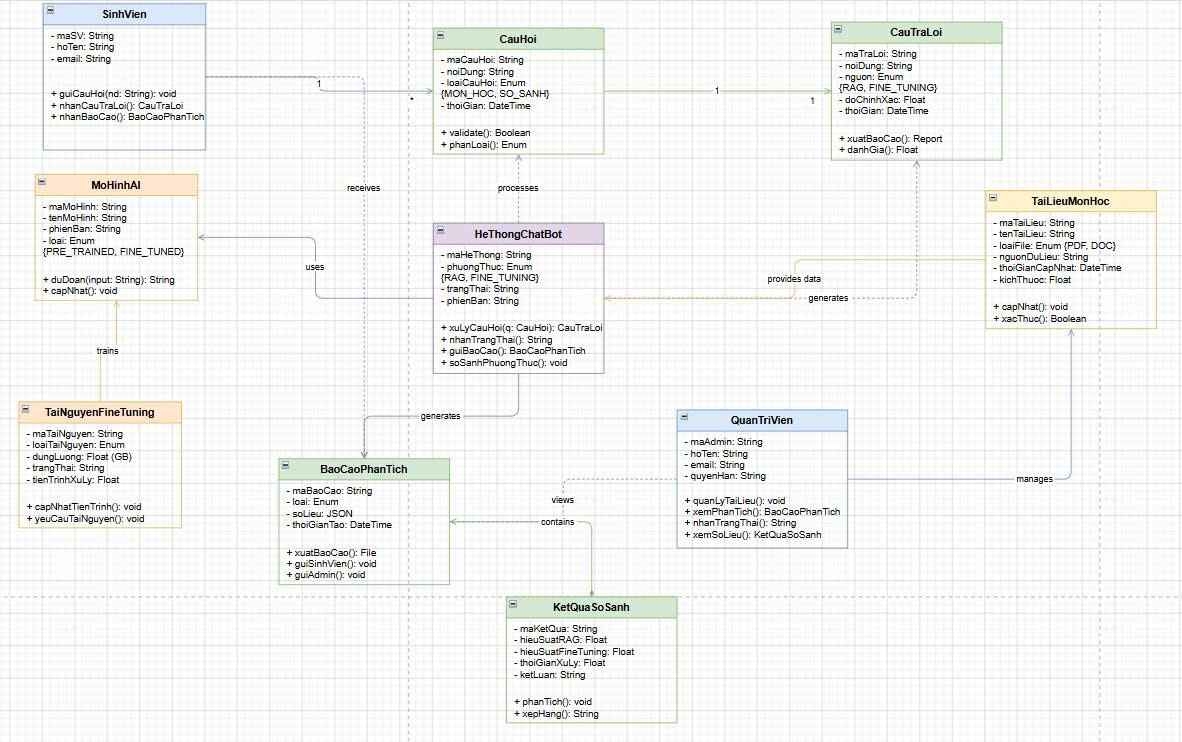
\includegraphics[width=\textwidth]{images/class_diagram.png}
	\caption{Biểu đồ lớp của hệ thống}
	\label{fig:class}
\end{figure}

Biểu đồ lớp gồm các lớp chính sau:

\subsection*{SinhVien}

Đại diện cho người sử dụng hệ thống.

Các chức năng:

\begin{itemize}
	\item Gửi câu hỏi.
	\item Nhận câu trả lời.
	\item Nhận báo cáo đánh giá.
\end{itemize}

Sinh viên là tác nhân trực tiếp tương tác với hệ thống Chatbot.

\subsection*{CauHoi}

Lưu toàn bộ thông tin câu hỏi do người dùng gửi lên.

Bao gồm:

\begin{itemize}
	\item Nội dung câu hỏi.
	\item Loại câu hỏi.
	\item Môn học.
	\item Thời gian gửi.
\end{itemize}

Sau khi tiếp nhận, câu hỏi sẽ được chuyển tới lớp HệThốngChatbot để xử lý.

\subsection*{HeThongChatbot}

Đây là lớp trung tâm của hệ thống.

Các nhiệm vụ chính:

\begin{itemize}
	
	\item Điều phối quá trình xử lý.
	
	\item Chọn RAG hoặc Fine-Tuning.
	
	\item Gọi mô hình AI.
	
	\item Sinh báo cáo.
	
	\item So sánh hai phương pháp.
	
\end{itemize}

Mọi thành phần đều kết nối thông qua lớp này.

\subsection*{MoHinhAI}

Đại diện cho các mô hình AI bên ngoài.

Ví dụ:

\begin{itemize}
	
	\item Gemini
	
	\item GPT
	
	\item Llama
	
\end{itemize}

Hệ thống gửi Prompt và nhận câu trả lời từ mô hình AI.

\subsection*{TaiLieuMonHoc}

Quản lý toàn bộ tài liệu PDF, DOCX và TXT.

Tài liệu sau khi tải lên sẽ được chia nhỏ (Chunking) và lưu vào ChromaDB để phục vụ RAG.

\subsection*{TaiNguyenFineTuning}

Lưu các tài nguyên phục vụ Fine-Tuning như:

\begin{itemize}
	
	\item Dataset
	
	\item GPU
	
	\item Dung lượng
	
	\item Thời gian xử lý
	
\end{itemize}

\subsection*{BaoCaoPhanTich}

Lưu toàn bộ kết quả đánh giá.

Bao gồm:

\begin{itemize}
	
	\item Accuracy
	
	\item Thời gian phản hồi
	
	\item Chi phí
	
	\item Kết luận
	
\end{itemize}

\subsection*{KetQuaSoSanh}

Thực hiện so sánh giữa RAG và Fine-Tuning dựa trên nhiều tiêu chí khác nhau.

\subsection*{QuanTriVien}

Quản lý:

\begin{itemize}
	
	\item Người dùng
	
	\item Tài liệu
	
	\item Báo cáo
	
	\item Trạng thái hệ thống
	
\end{itemize}

\section{Thiết kế cơ sở dữ liệu}

Hệ thống sử dụng cơ sở dữ liệu quan hệ để quản lý thông tin người dùng, tài liệu, câu hỏi và báo cáo đánh giá.

\begin{figure}[H]
	\centering
	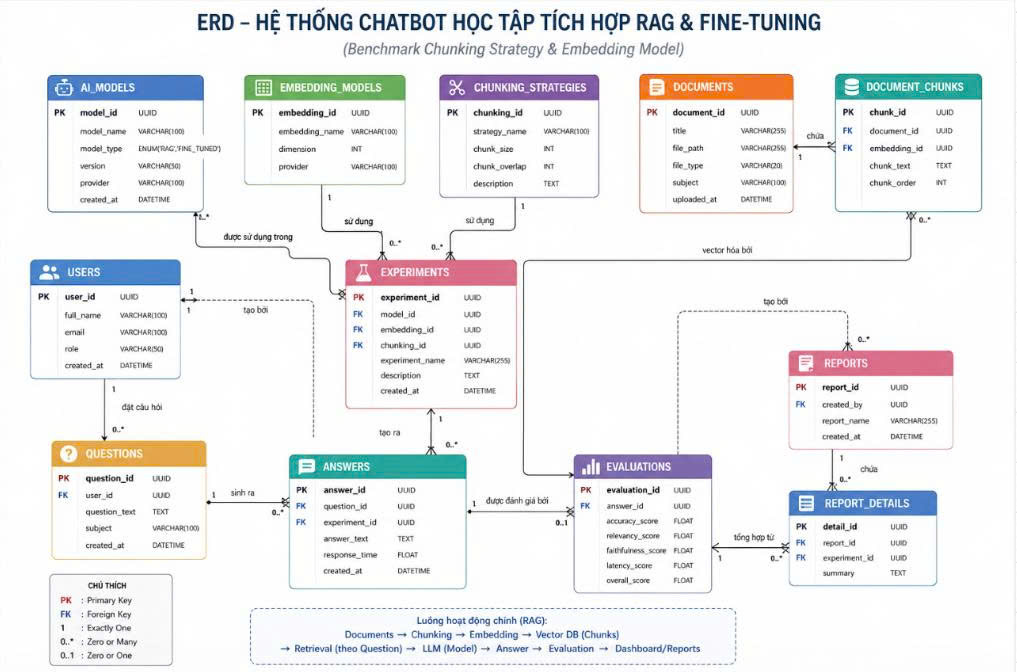
\includegraphics[width=\textwidth]{images/erd.png}
	\caption{ERD của hệ thống}
	\label{fig:erd}
\end{figure}

ERD mô tả toàn bộ các bảng dữ liệu phục vụ hệ thống.

\subsection*{Users}

Lưu thông tin sinh viên và quản trị viên.

\subsection*{Questions}

Lưu lịch sử câu hỏi của người dùng.

Mỗi câu hỏi thuộc về một người dùng.

\subsection*{Answers}

Lưu câu trả lời do AI sinh ra.

Mỗi câu trả lời gắn với một câu hỏi.

\subsection*{Documents}

Lưu thông tin tài liệu gốc.

Bao gồm:

\begin{itemize}
	
	\item Tên tài liệu
	
	\item Đường dẫn
	
	\item Môn học
	
	\item Ngày tải lên
	
\end{itemize}

\subsection*{Document Chunks}

Lưu các đoạn văn sau khi Chunking.

Đây là dữ liệu được đưa vào ChromaDB.

\subsection*{Embedding Models}

Quản lý các mô hình Embedding.

Ví dụ:

\begin{itemize}
	
	\item BAAI
	
	\item Sentence Transformer
	
	\item OpenAI Embedding
	
\end{itemize}

\subsection*{Chunking Strategies}

Lưu chiến lược chia nhỏ tài liệu.

Ví dụ:

\begin{itemize}
	
	\item Fixed Size
	
	\item Recursive
	
	\item Semantic Chunking
	
\end{itemize}

\subsection*{Experiments}

Lưu từng lần chạy thử nghiệm giữa RAG và Fine-Tuning.

\subsection*{Evaluations}

Lưu các chỉ số đánh giá:

\begin{itemize}
	
	\item Accuracy
	
	\item Relevancy
	
	\item Latency
	
	\item Faithfulness
	
\end{itemize}

\subsection*{Reports}

Lưu báo cáo tổng hợp cuối cùng của từng lần thử nghiệm.

\section{Luồng xử lý dữ liệu}

Khi người dùng gửi câu hỏi, hệ thống sẽ thực hiện theo các bước sau:

\begin{enumerate}
	
	\item Tiếp nhận câu hỏi từ giao diện React.
	
	\item FastAPI nhận Request.
	
	\item Kiểm tra chế độ RAG hoặc Fine-Tuning.
	
	\item Nếu là RAG:
	
	\begin{itemize}
		
		\item Chunking tài liệu.
		
		\item Embedding.
		
		\item Truy vấn ChromaDB.
		
		\item Sinh Prompt.
		
		\item Gửi tới LLM.
		
	\end{itemize}
	
	\item Nếu là Fine-Tuning:
	
	\begin{itemize}
		
		\item Gửi trực tiếp tới mô hình đã huấn luyện.
		
	\end{itemize}
	
	\item Nhận câu trả lời.
	
	\item Ghi lịch sử.
	
	\item Trả kết quả về giao diện.
	
\end{enumerate}

\section{Kết luận chương}

Chương này đã trình bày chi tiết thiết kế hệ thống Chatbot từ góc nhìn hướng đối tượng và cơ sở dữ liệu. Class Diagram mô tả các lớp và mối quan hệ giữa các thành phần, trong khi ERD thể hiện cấu trúc dữ liệu phục vụ cho quá trình lưu trữ và xử lý. Những thiết kế này là nền tảng để triển khai hệ thống ở chương tiếp theo.